\section{Methodology}
\label{sec:methodology}

In this work, we adapt a pre-trained video generation model for video reshooting. This task requires modifying the camera trajectory of an existing video while preserving its core content and visual style. We first define the overall task, then describe our novel self-supervised data pipeline, and finally detail the architectural adaptations and training augmentations required to implement our approach.




\begin{figure*}
    \centering
    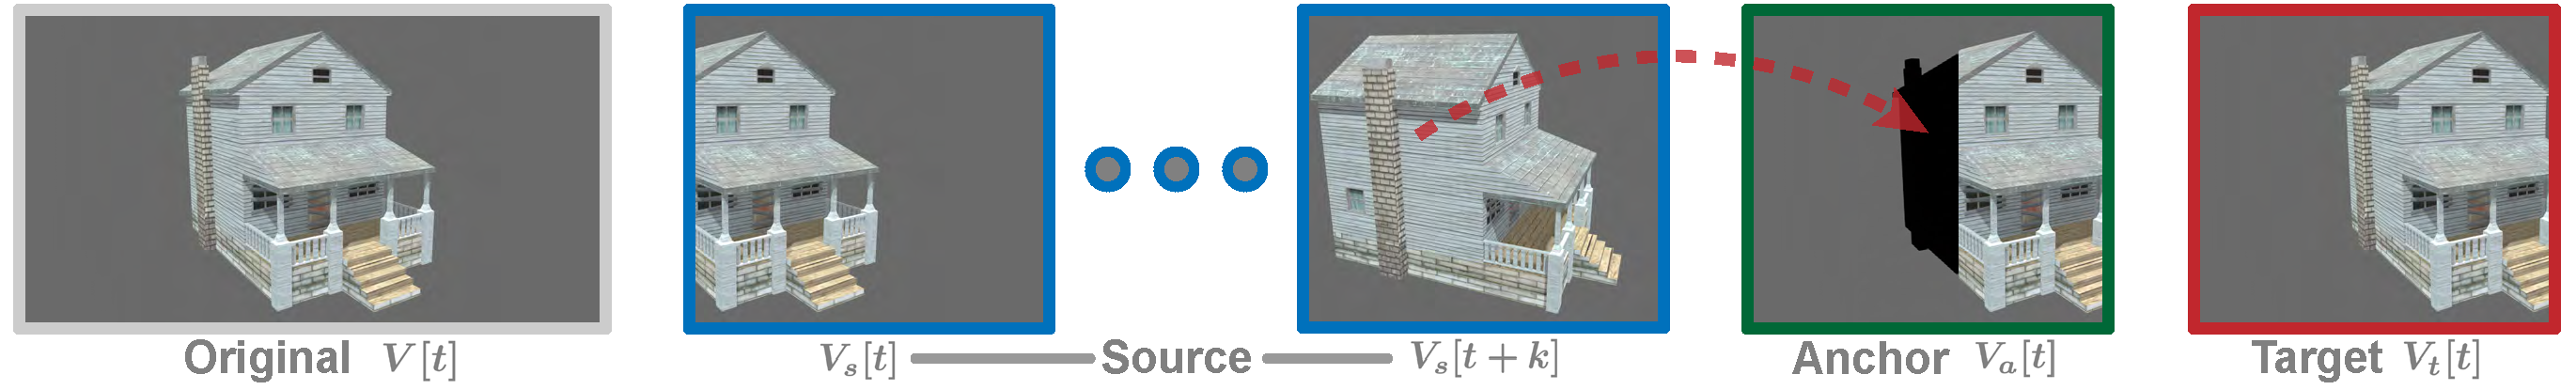
\includegraphics[width=0.8\linewidth]{figures/impl_reprojection.pdf}
    \vspace{-0.1in}
    \caption{
    \textbf{Implicit Spatiotemporal Reasoning in our Self-Supervised Setup.}
    Our training method forces the model to learn spatial structure from 2D data. To reconstruct the target $V_t$ at frame $t$, the model is given the disoccluded anchor $V_a[t]$. The corresponding source frame $V_s[t]$ may not contain the missing texture (e.g., the side of the building). The model is forced to find this texture in a different source frame, $V_s[t+k]$, where it is visible due to $V_s$'s independent camera motion. While this example shows a static 3D building for simplicity, performing this routing on dynamic videos forces the model to learn the scene's underlying complex 4D interactions.
    }
    \label{fig:implicit_3d}
    \vspace{-0.2in}
\end{figure*}


The video reshooting task requires synthesizing a high-fidelity target video ($V_{t}$) based on a new desired camera path. At inference time, our model is conditioned on two primary inputs: the source video ($V_{s}$), which serves as the high-quality texture and content reference, and the anchor video ($V_{a}$), which defines the target camera motion. This anchor video is typically pre-rendered from a 4D representation of the original scene.

Following recent approaches~\cite{yu2025trajectorycrafter,ex4d,jeong2025reangle,bai2024syncammaster,wang2025epic}, we utilize an anchor video as a primary conditioning signal. This choice is crucial for two main reasons:
\begin{description}[noitemsep, topsep=0pt, partopsep=0pt, leftmargin=0pt, style=unboxed, font=\normalfont\bfseries]
    \item [Intuitive Visual Guidance:] An anchor video offers a dense, intuitive visual representation of the target camera trajectory, which is empirically more effective for guiding generative models than explicit camera poses~\cite{wang2025epic}.
    \item [Self-Supervised Training Necessity:] It is essential for our novel self-supervised training strategy (Section~\ref{sec:self_supervision}). Our method generates pseudo-views from 2D crops without modifying underlying 3D camera parameters, making relative camera poses non-viable. The anchor provides the concrete spatiotemporal target needed for our pseudo multi-view pairs.
\end{description}

While the anchor video ($V_a$) is crucial for defining the target trajectory, it is inherently imperfect, suffering from artifacts like holes and inaccuracies caused by depth and pose estimation errors. The model's core task is to generate $V_{t}$ that faithfully follows the motion of $V_{a}$ while replacing its distorted content with clean, temporally consistent textures sourced from $V_{s}$. Training this two-stream model ideally requires large-scale triplets $(V_{s}, V_{a}, V_{t})$ with pristine $V_t$ ground-truth, which is logistically intractable. We address this with our novel self-supervised approach, generating these triplets from monocular videos alone.



\subsection{Self-Supervision from Monocular Video}
\label{sec:self_supervision}

To bypass the challenges of paired multi-view data acquisition, we synthesize the required $(V_s, V_a, V_t)$ training triplets solely from abundant monocular videos.

\subsubsection{Pseudo-View Triplet Generation}
\label{sec:pseudo_view_triplet}

From a single input video $V$, we employ a smooth video cropper to generate two distinct clips. These clips will form our source video ($V_s$) and target video ($V_t$). Each clip follows an independent smooth random-walk trajectory that emulates dynamic camera motion, as shown in Fig.~\ref{fig:teaser}. Each trajectory is generated by sampling an adaptive number of random control points within the frame boundaries, with the overall motion magnitude governed by a tunable scale parameter. A natural cubic spline is then fitted through these control points to produce a continuous crop trajectory.


We sample two trajectories using different random seeds, resulting in clips $(V_{s}, V_{t})$ that observe different regions of the same video. Because they are drawn from the same source, this effectively mimics time-synchronized distinct moving cameras. Importantly, the original video $V$ may already exhibit its own inherent camera motion. Our method naturally inherits this, capturing complex patterns such as orbits, pans, and zooms from in-the-wild footage.

Based on both clips, we synthetically generate the anchor video ($V_{a}$) to complete the training triplet. We generate $V_{a}$ by warping the first frame of the source video ($V_{s}[0]$) to align with the target video's trajectory ($V_{t}$). This warping process, illustrated in Fig.~\ref{fig:triplets}, is guided by an offset-aware flow field combining a dense tracking field (capturing 2D pixel motion) with a crop offset flow (capturing the change in pseudo-viewpoint). To obtain the dense tracking field, we use AllTracker~\cite{4d_recon_harley2025alltracker} on the original video $V$ before cropping, leveraging all intermediate frames for robust temporal correspondences. This combined flow is then used to forward-warp $V_{s}[0]$ over time using softmax splatting~\cite{softmax_splatting}:
\begin{equation}
V_{a}[t] = \text{SoftSplat}(V_s[0], F_{\text{comb}}(t)),
\label{eq:anchor_warping}
\end{equation}
where $V_a[t]$ is the $t$-th frame of the anchor video, $\text{SoftSplat}$ is the forward warping operator, and $F_{\text{comb}}(t)$ is our combined offset-aware flow field.  The use of forward warping is a deliberate choice, effectively simulating the artifacts, occlusions, and dis-occlusions characteristic of the point-cloud-based anchor videos used at inference.




\begin{figure*}
    \centering
    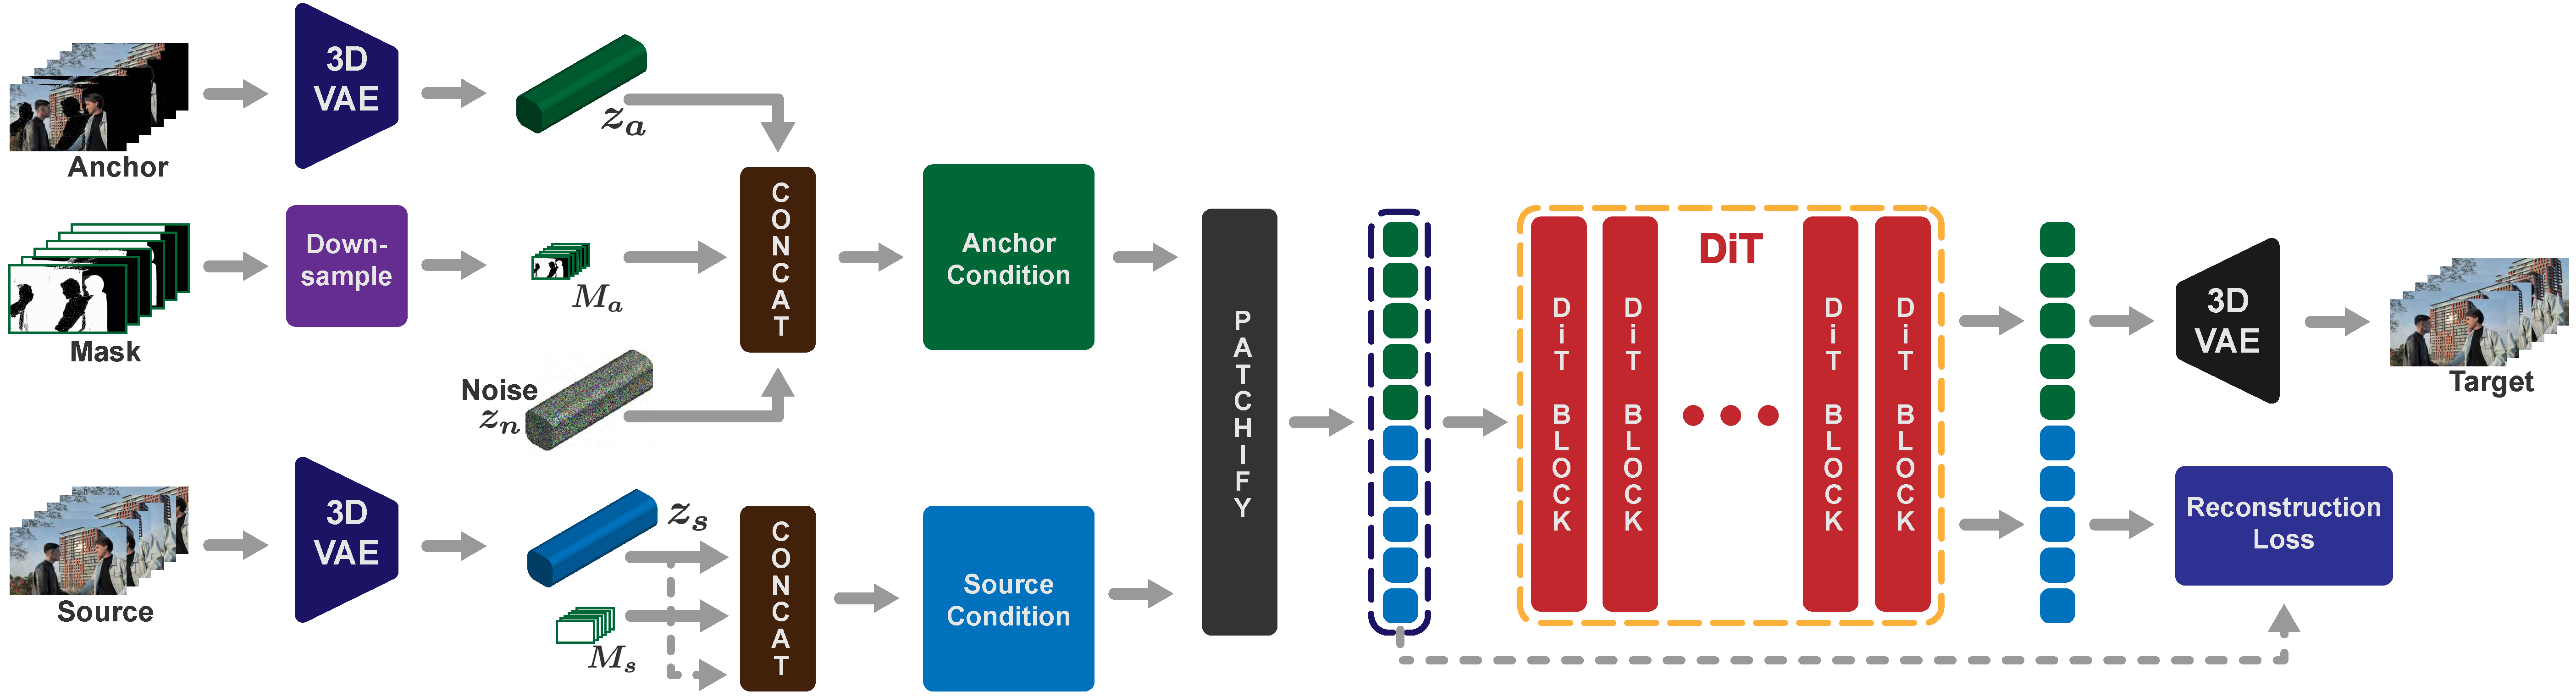
\includegraphics[width=0.8\linewidth]{figures/overview.pdf}
    \vspace{-0.13in}
    \caption{\textbf{Overview of our Conditioning Architecture.} Our model adapts a pre-trained DiT-based I2V model~\cite{wan21}. \textbf{(1) VAE Encoding:} The Anchor video ($V_a$) and Source video ($V_s$) are independently encoded into latents by the VAE ($z_a, z_s$). \textbf{(2) Conditioning Setup:} The Anchor latent ($z_a$) is combined with a noise latent ($z_{n}$) and its corresponding mask ($M_a$). The Source latent ($z_s$) is duplicated (replacing $z_{n}$) and combined with an all-ones mask ($M_s$). \textbf{(3) DiT Processing:} The two conditioned streams are temporally concatenated and fed into the DiT blocks. \textbf{(4) Source Token Management \& Denoising:} After each denoising step, the output tokens corresponding to the Source are subjected to an auxiliary reconstruction loss (ensuring source content retention).}
    \label{fig:overview}
    \vspace{-0.2in}
\end{figure*}


\subsubsection{Implicit 4D-Aware Learning}
\label{sec:implicit_4d_learning}

This training setup directly forces the model to learn its inference-time task. It must reconstruct the high-quality, dynamic $V_{t}$ by mastering the following sub-tasks:

\begin{description}[noitemsep, topsep=0pt, partopsep=0pt, leftmargin=0pt, style=unboxed, font=\normalfont\bfseries]
    \item[Ignoring Anchor Artifacts] The model learns to treat $V_{a}$ strictly as a geometric guide, ignoring warping artifacts and relying on it only for structure.
    \item[Temporal Synchronization of Dynamics] By training on perfectly synchronized pseudo-views of real-world events, the model natively learns to map complex non-rigid motion frame-by-frame. This directly solves the synchronization failures commonly seen in models trained purely on synthetic data or static-dynamic split datasets.
    \item[Spatial Content Sourcing] The model is forced to find the correct, high-fidelity textures from $V_{s}$. Because $V_{s}$ and $V_{t}$ are not spatially aligned, the model must use its attention mechanism to route content from different spatial regions of the source.
    \item[Implicit 4D Reconstruction] As shown in Fig.~\ref{fig:implicit_3d}, generating a target frame often reveals hidden areas that are not visible in the corresponding source frame. To fill these missing regions, the model must search through the source video to find the required texture in a different frame. It then stitches this temporal information into the correct spatial position. While Fig.~\ref{fig:implicit_3d} illustrates this concept on a static building for simplicity, applying this "search and stitch" process to videos of moving subjects forces the model to track geometry across both space and time. This fundamentally teaches the model implicit 4D reconstruction.
    \item[Generative In-painting] For regions not visible in any $V_{s}$ frame, the model learns to leverage its generative priors to plausibly hallucinate the missing details.
\end{description}

This self-supervised strategy has key advantages over synthetic or 3D-annotated approaches. Our entire data pipeline relies only on a robust 2D dense tracker, making it domain-agnostic and applicable to virtually any monocular video. As a result, we can train on a vast corpus that includes photorealistic footage, animation, and generative art, exposing the model to diverse camera motions without restrictive domain limitations. Importantly, our training objective does not directly optimize for explicit 4D reconstruction; rather, dynamic 4D re-rendering emerges as a learned capability to solve this complex 2D-based routing task.



\subsection{Model Architecture and Conditioning}
\label{sec:architecture}


Having established our self-supervised training data (Section~\ref{sec:self_supervision}), we now detail the architectural adaptations required to finetune a pre-trained video diffusion model for our task, as illustrated in Figure~\ref{fig:overview}.

\subsubsection{Video Diffusion Models and DiT Conditioning}
\label{sec:arch_background}

Our approach adapts the WAN 2.2 I2V architecture~\cite{wan21}, a Diffusion Transformer (DiT). The base model is trained to predict the denoised latent from a noisy input, effectively reversing the diffusion process to generate high-quality frames. Conditional signals in DiT architectures can be integrated via channel concatenation, dedicated cross-attention layers, or as supplementary tokens processed by the full self-attention mechanism~\cite{bai2025recammaster, peebles2023scalable}. The chosen mechanism is critical for temporal modeling and Rotary Positional Embeddings (RoPE), which encode relative spatiotemporal positional information~\cite{bai2025recammaster, su2024roformer}. We leverage a token-based conditioning approach as detailed below.

\subsubsection{Source-Anchor Fusion with Offset RoPE}
\label{sec:offset_rope}

Our model leverages an anchor video ($V_a$) for geometric guidance and a source video ($V_s$) for high-fidelity texture. Instead of utilizing separate cross-attention layers for $V_s$, which often proves ineffective for this task~\cite{bai2025recammaster}, we process both $V_s$ and $V_a$ as tokens within the model's main self-attention mechanism.

Both $V_a$ and $V_s$ are independently encoded into latents ($z_a, z_s$) by the VAE. The Anchor condition combines $z_a$ with a noise latent ($z_n$) and its downsampled binary mask ($M_a$). The Source condition uses $z_s$ with an all-ones mask ($M_s$), ensuring all content is leveraged. These two prepared conditional streams are then temporally concatenated and fed into the DiT blocks.

Within each DiT block, 3D RoPE is applied. To enable robust flexible-length video generation, we implement an Offset RoPE. A large, fixed offset is applied only to the temporal positional embeddings of the $V_s$ tokens, effectively decoupling the source condition's perceived position from the target's temporal position. While output source tokens do not directly form $V_t$, an auxiliary reconstruction loss is applied during training between the output source tokens and their original clean latents ($z_s$). This encourages the source pathway to preserve high-fidelity content from $V_s$.




% \begin{table*}[t]
% \label{table-main-comparison}
% 	\begin{center}
% \vspace{-0.30cm}
% 		\caption{Quantitative comparison with SOTA methods on VBench, temporal consistency, camera accuracy, and view synchronization.}
% \vspace{-0.30cm}
% 		\label{tab_merged_eval}
% 		\setlength\tabcolsep{3.2pt} % Keep small for fitting
%  	\centering
%  	\resizebox{\textwidth}{!}{ % Use \textwidth to fit the wide table
% 		\begin{tabular}{lcccccc|c|cc|ccc}
% 			\toprule
% 			\multirow{2}{*}{Method}
%             & \multicolumn{6}{c|}{VBench Quality}
%             & \multicolumn{1}{c|}{Temporal Consistency}
%             & \multicolumn{2}{c|}{Camera Accuracy}
%             & \multicolumn{3}{c}{View Synchronization} \\
%      	\cmidrule(lr){2-7}
%      	\cmidrule(lr){8-8}
%      	\cmidrule(lr){9-10}
%      	\cmidrule(lr){11-13}
%             & \makecell[c]{Aesthetic $\uparrow$} & \makecell[c]{Imaging $\uparrow$} & \makecell[c]{Flickering $\uparrow$} & \makecell[c]{Smoothness $\uparrow$} & \makecell[c]{Subject $\uparrow$} & \makecell[c]{Background $\uparrow$}
% 			& CLIP-F $\uparrow$
% 			& RotErr $\downarrow$
% 			& TransErr $\downarrow$
% 			& Mat. Pix $\uparrow$
% 			& FVD-V $\downarrow$
% 			& CLIP-V $\uparrow$ \\
% 		\midrule

% 	\trajectorycrafter{} (49 frames) & 52.69 & \textbf{59.67} & 96.97 & 99.03 & 93.78 & 95.13 & 98.80 & \textbf{2.26} & 3.03 & 1851.80 & 582.56 & 92.40 \\
% 	\textbf{Ours} (49 frames) & \textbf{52.72} & 57.81 & \textbf{97.43} & 99.24 & 95.09 & 95.62 & 99.01 & 2.61 & 2.73 & 2737.65 & 488.22 & 94.96 \\
%     \midrule
% 	\recammaster{} & 48.71 & 52.61 & \textbf{97.57} & \textbf{99.26} & 88.57 & 90.65 & 98.49 & 11.29 & 19.59 & 1314.00 & 732.52 & 88.91 \\
% 	\exfd{} & 49.72 & 55.76 & 97.46 & 99.08 & 91.51 & 94.78 & 98.94 & 3.94 & \textbf{4.21} & 2188.98 & 685.63 & 89.77 \\
% 	% \textbf{Ours} & 53.05 & 58.39 & 97.42 & 99.20 & \textbf{93.43} & 95.11 & 99.04 & 3.27 & 4.92 & 2636.07 & 595.39 & 92.94 \\
%     \midrule
%     \textbf{Ours w/o Source Video} & \textbf{53.97} & \textbf{58.92} & 97.13 & 98.99 & 93.12 & 95.03 & 98.95 & 4.82 & 11.65 & 226.01 & 662.09 & 89.97 \\
%     \textbf{Ours} & 52.85 & 58.64 & 97.37 & 99.21 & 93.43 & 95.24 & 99.03 & 2.76 & 4.23 & \textbf{2720.83} & \textbf{586.24} & \textbf{93.16} \\
% \bottomrule
% 		\end{tabular}
%  	}
% 	\end{center}

%     \vspace{-0.33in}
% \end{table*}



\begin{figure}
    \centering
    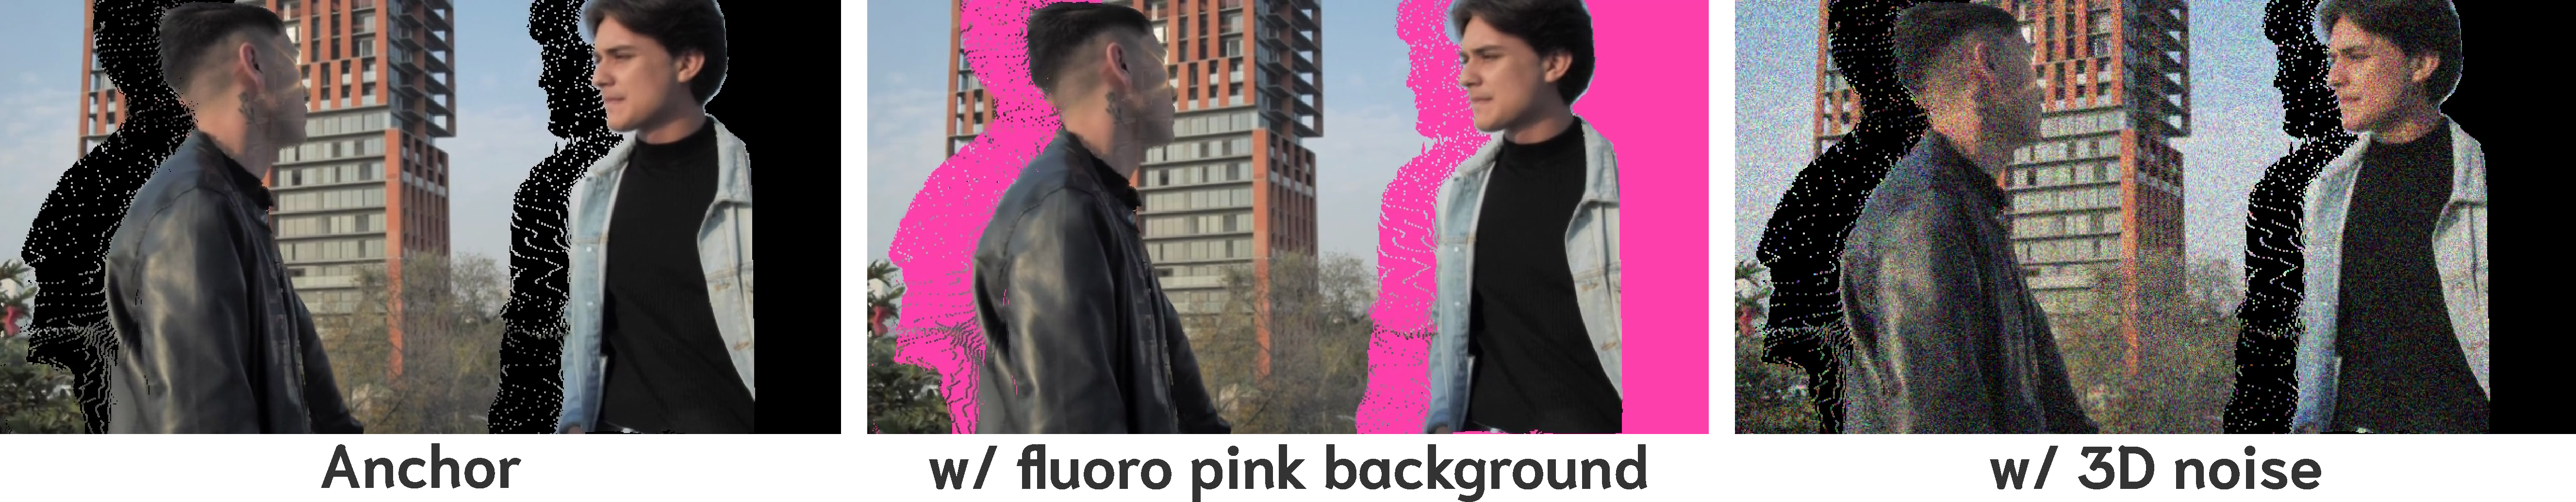
\includegraphics[width=\linewidth]{figures/ablations_input.pdf}
    \vspace{-0.25in}
    \caption{This figure demonstrates key augmentations applied during Anchor Video ($V_a$) generation, shown on a single frame. From left to right: the default anchor with a black masked background; an anchor using a fluorescent pink background for masked regions; and an anchor with 3D-aware noise coherently injected into its reference frame. These techniques improve model robustness and help mitigate artifacts in challenging scenes (Section~\ref{sec:technical_augmentations}).}
    \label{fig:ablations_input}
    \vspace{-0.2in}
\end{figure}




\begin{figure*}
    \centering
    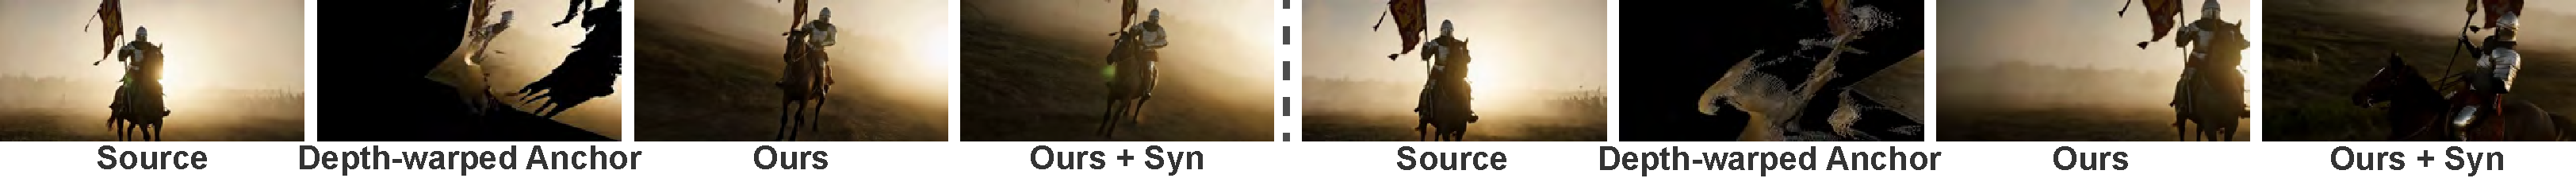
\includegraphics[width=\linewidth]{figures/data_ablation.pdf}
    \vspace{-0.27in}
    \caption{
        We evaluate models trained with (Ours + Syn) and without (Ours) the 15\% synthetic data mixture. \textbf{Left:} Under moderate camera motion, both models successfully follow the anchor video, demonstrating that our self-supervised monocular pipeline natively learns robust 4D structures. \textbf{Right:} For extreme out-of-distribution camera rotations, the monocular-only model struggles to align with the anchor. Conversely, the hybrid model accurately follows the extreme trajectory while preserving high-fidelity textures, confirming the synthetic mixture provides important priors for extreme 6DoF camera generalization.
    }
    \label{fig:hybrid_ablation}
    \vspace{-0.25in}
\end{figure*}


\subsubsection{Technical Augmentations for Robust Training}
\label{sec:technical_augmentations}

Beyond our core architecture, we integrate several technical augmentations to enhance robustness against inference-time artifacts (Fig.~\ref{fig:ablations_input}). Detailed configurations are provided in the Supplementary Material.

\begin{description}[noitemsep, topsep=0pt, partopsep=0pt, leftmargin=0em, style=unboxed, font=\normalfont\bfseries]
    \item[Source Token Reconstruction Loss] An auxiliary loss applied to ensure content retention from the source video.
    \item[Fluorescent Anchor Background] We use a high-contrast background, such as fluorescent pink, in masked-out regions of the anchor video to provide a clear boundary signal. This is specially effective for dark scenes.
    \item[Random Anchor Reference Frame Warping] Randomly selecting the reference frame for anchor warping prevents model bias towards early frames.
    \item[3D-Aware Noise] Gaussian noise is applied directly to the anchor's reference frame prior to warping. This noise moves coherently with the underlying structure, suppressing simple texture copying from anchor while strictly preserving geometric guidance.
\end{description}



